\documentclass[10pt]{article}
\usepackage[utf8]{inputenc}

\title{IF679- Informática e Sociedade}
\author{Jose Guilherme Nascimento Vieira da Silva}
\date{Maio 2019}

\usepackage{natbib}
\usepackage{graphicx}
\usepackage[brazil]{babel}
\usepackage{url}

\begin{document}

\maketitle

\section{Introdução}
A cadeira de Informática e Sociedade é uma disciplina que combina o estudo da sociologia com um aprofundamento do impacto da tecnologia na mesma\cite{ProgramaInfosoc}. Esse curso traz para debate dilemas
enfrentados por nossa sociedade com a intenção de desenvolver nos alunos o pensamento crítico necessário para que as mudanças realizadas pelo mesmos sejam pensadas para melhor bem-estar dos usuários, respeitando códigos de ética convencionados pelos grupos de pessoas que usam o sistema e os impactos positivos e negativos da tecnologia criada. Nesse semestre a cadeira é ofertada pelas professoras Veronica
Teichrieb
e Carina Frota Alves nas quartas e sextas no turno da manhã \cite{PetInfosoc}.

A disciplina tem 3 pilares:
   \begin{figure}
   \begin{center}
    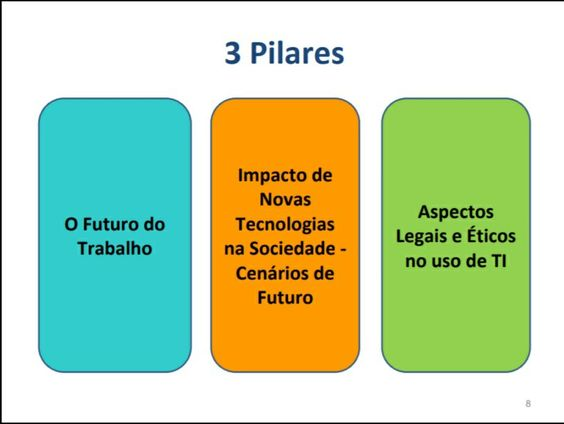
\includegraphics[scale=0.3]{jgnvs.jpg}   
   \end{center}
   \end{figure}

\begin{itemize}
    \item \textbf{Processos de Software}: um conjunto estruturado de atividades, procedimentos, artefatos e ferramentas necessários para o desenvolvimento de um sistema de software;

    \item \textbf{Futuro do Trabalho}: Discussões sobre como a
tecnologia impacta nos empregos atuais, como ela pode criar novas profissões, mudar a ideia de trabalho e quais podem ser as competências do futuro;
        
    \item \textbf{Impacto de Novas Tecnologias na Sociedade - Cenários de Futuro}: Tecnologia sendo usada em diferentes meios, inovações radicais, entender necessidades de diferentes usuários e desafios para as futuras gerações;
    
    \item \textbf{Aspectos Legais e Éticos no uso de TI}: Privacidade, ética, marco civil da internet, direitos autorais, neutralidade da rede entre outras temas atuais.
    
\end{itemize}

\section{Relevância}
A cadeira de informática e Sociedade está no currículo do curso de ciências
e engenharia da computação e surge da necessidade de apresentar aos alunos a importância da tecnologia na sociedade atual e como ela impacta no ambiente que se apresenta. A mesma tem um perfil diferente da maioria das cadeiras no CIn
, fugindo da matemática, lógica e programação. E por apresentar o outro lado da computação, ou seja, os usuários, ela se mostrar uma cadeira que prepara os alunos para o mundo real no qual terão que lidar o tempo todo com as necessidades dos usuários.

\section{Relação com outras disciplinas}
Durante a cadeira há muitas discussões e rodas de conversa relacionadas ao impacto da tecnologia na sociedade, portanto, na minha opinião, as seguintes cadeiras tem relação com essa disciplina:

\begin{table}[h]
\resizebox{12.1cm}{!}{
\begin{tabular}{l|l}
\textbf{Cadeiras}                      & \textbf{Motivo}                                        \\ \hline
IF-668 Introdução à Computação & Discussões relacionadas ao impacto da computação na sociedade \\
IF-676 Metodologia e Expressão Técnico-Científica  & Preocupação maior de que as pesquisas e textos sigam modelos acadêmicos \\
IF-683- Projeto de Desenvolvimento (Projetão) & Intensifica compreensão de como mudar um ambiente com tecnologia e impacto da mesma. 
\end{tabular}}
\end{table}

\bibliographystyle{plain}
\bibliography{jgnvs.bib}
\end{document}

